\section{Gas-Filled Detectors} 
%{\color{red} This section still needs to be done!!!}
\subsection{Overview}
\subsubsection{Transportation of Charged Particles in Gases}
\begin{itemize}
    \item Radiation excites and ionizes gases. Per every electron-ion pair created, 30$\sim$35 eV is lost. Without an external electric field, the charges would simply recombine; with the external electric field, particles of opposite charges would drift in opposite directions, resulting in a measurable electric current. 
    \item After the charged particles form, they can undergo various interaction mechanisms with one another or neutral atoms / molecules. The charged particles can participate in random thermal motion and diffuse. During diffusion, the electron may attach to a neutral gas molecule and form a negatively charged ion. Charge transfer motion, where electrons of a neutral molecule are transferred to a positive ion, can also occur; this is especially evident in gas mixtures of various ionization energies. Recombination can also occur when positive ions catch free electrons, or when positive ions and negative ions meet (latter more prominent). 
    \item There are two main types of recombination loss:
    \begin{itemize}
        \item Columnar (initial) recombination:\\
        Ion pairs are formed in a column along the track of the ionizing particle, leading to high local density of ion pairs. This is especially severe for densely ionizing particles such as heavy-charged particles, whose track is shorter in comparison to, say, fast electrons. 
        \item Volume recombination:\\
        Volume recombination occurs when oppositely charged particles meet after they have left their initial position, the aforementioned track. Volume recombination increases with higher irradiation rate, and is therefore combated with higher electric fields. (This feature can be seen in figure~\ref{fig:ion_chamber_saturation_current}.)
    \end{itemize}
    \item An external electric field $E$ ``drifts'' charges to electrodes. The total motion of charges is the superposition of drift and thermal motion.
    \begin{itemize}
        \item The drift velocity is given by $v=\mu E/p$, where $E$ is the electric field strength, $p$ is the gas pressure, and $\mu$ is mobility.
        \item Typical values of $\mu$ fall between $1\sim1.5\times10^{-4}\;m^2s\;atm$\\
        (if $p=1\;atm$ and $E=10^4\;V/m$, then $v\approx1\;m/s$)
        \item Electrons have $\approx1000\times$ higher mobility than ions due to its light mass.
    \end{itemize}
\end{itemize}
\subsubsection{Operational Modes}
\begin{figure}[ht]
    \centering
    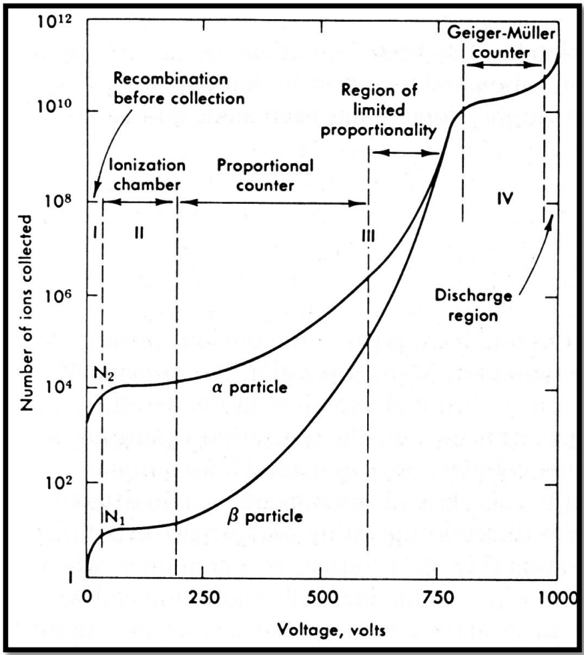
\includegraphics[width=0.5\textwidth]{images/gas_detector_operation_modes.png}
    \caption{Operational modes of gas detectors.}
    \label{fig:gas_detector_operation_modes}
\end{figure}
As shown in figure~\ref{fig:gas_detector_operation_modes}, from low to high voltage, operational modes include (for regions 2, 3, and 5, see following sections for detailed discussions):
\begin{enumerate}
    \item Recombination region (recombination before collection):\\
    Incomplete charge collection
    \item Ionization region (ionization chamber):
    \begin{itemize}
        \item Complete primary charge collection, without multiplication or amplification.
        \item Collected charge is proportional to energy, but signals are small. 
        \item Typically used for heavy charged particle detection or when there are fluxes of radiation.
    \end{itemize}
    \item Proportional counter (proportional counter):
    \begin{itemize}
        \item With electron energies larger than ionization energies, charge multiplication (secondary charge generation) occurs. Signals are amplified by $\approx 10^6$.
        \item Below $\approx600\;V$, the signal amplitude / charge is proportional to energy.
    \end{itemize}
    \item Region of limited proportionality:\\
    Above $\approx600\;V$, due to space charge effects, where positive ions reduce the electric field, there is limited proportionality. 
    \item Geiger-Müller region (GM counter):
    \begin{itemize}
        \item Secondary avalanches occur along the anode wire until the space charge is sufficient to reduce the electric field and suppress multiplication. 
        \item Signals independent of primary charges; no energy information is provided and is only a counter!
    \end{itemize}
    \item Discharge region:
    \begin{itemize}
        \item Continuous discharge occurs with or without radiation present.
        \item To be avoided since this damages the counter.
    \end{itemize}
\end{enumerate}
\subsection{Ionization Chamber}
\subsubsection{Current Mode Operation}
\begin{figure}[ht]
    \centering
    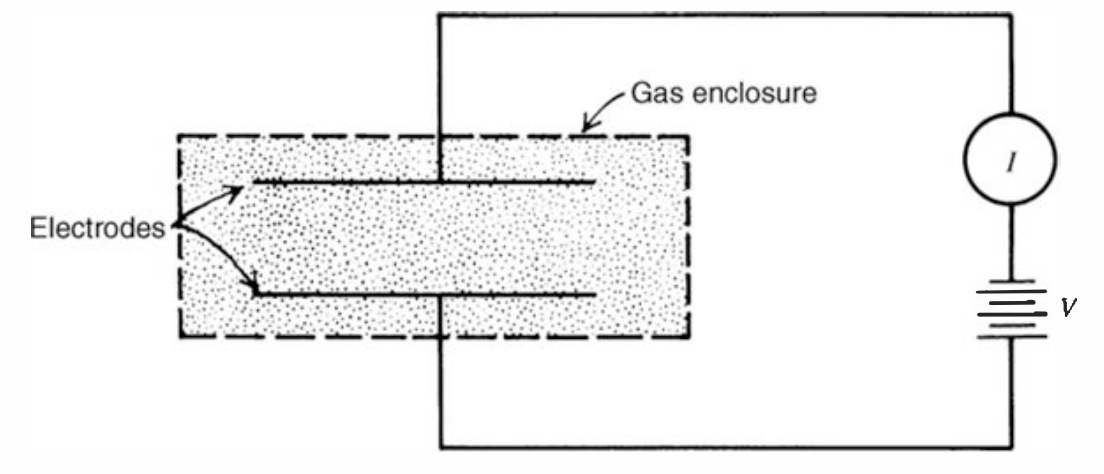
\includegraphics[width=0.5\textwidth]{images/ion_chamber_current_mode.png}
    \caption{Basic elements of an ion chamber.}
    \label{fig:ion_chamber_current_mode}
\end{figure}
\begin{itemize}
    \item The drift of positive and negative charges in an electric field constitutes an electric current. 
    \item As shown in figure~\ref{fig:ion_chamber_current_mode}, the detector is a capacitor with capacity $C$ and stored charge $Q=CV$\\
    The motion of charges in the electric field causes a drop in the stored energy\\ $dE_\text{int}=q_+dV_++q_-dV_-$\\
    which is balanced by the energy supplied by the external circuit\\
    $dE_\text{ext}=VdQ$\\
    $\Rightarrow\;i=\frac{dQ}{dt}=\frac{1}{V}\left(q_+\frac{dV_+}{dt}+q_-\frac{dV_-}{dt}\right)$\\
    With $\frac{dV_\pm}{dt}=\frac{dV_\pm}{dx}\frac{dx}{dt}=E_\pm v_\pm$ and $q_+=q_-=q_0$ , we get $i=\frac{q_0}{V}(v_+E_++v_-E_-)$
    \item The expression found above shows that the signal of an ion chamber is generated by the motion of charges in an electric field, not the arrival of charges at the electrodes.
    \item Assuming constant / steady state irradiation, a constant (saturation) current that reflects the ion pair formation rate will be observed.
    \item As shown in figure~\ref{fig:ion_chamber_saturation_current},as voltage increases, the rate at which the ion pairs are separated increases, and recombination is suppressed. The measured current therefore increases. At a sufficiently high voltage, virtually all recombination is suppressed, and increasing the voltage no longer increases the current since all charges are already collected and their rate of formation is constant. This is the region of ion saturation. 
    \item Due to the aforementioned effects of recombination, higher voltages are needed in the presence of heavy charged particles (columnar recombination) and high irradiation rates (volume recombination). While diffusion of charges will occur due to the existence of a gradient (the concentration of positive ions is greatest near the cathode, and the concentration of negative ions is greatest near the anode), its effects on the saturation current are practically negligible. 
    \item Some additional features of ion chambers include
    \begin{itemize}
        \item sensitivity to energy rate and dose
        \item the use of any fill gases, including those that form negative ions (If recombination is negligible, while the drift velocity of negative ions are thousands of times slower than electrons, they create higher equilibrium concentration of negative charges, and the ion current end up being equal since it is the product of charge density and drift velocity.)
        \item small ion currents and high voltages, resulting in the need of high-quality insulators, guard rings (reduce insulator leakage), and low-noise amplifiers. (1 MeV radiation creates only 0.005 pC of charge)
    \end{itemize}
    \item Ion chambers are used as environmental monitors, survey meters, smoke detectors,  pocket dosimeters, etc., and for measurements of long half-lives, detection of ambient radioactive gases, etc. 
\end{itemize}
\begin{figure}[ht]
    \centering
    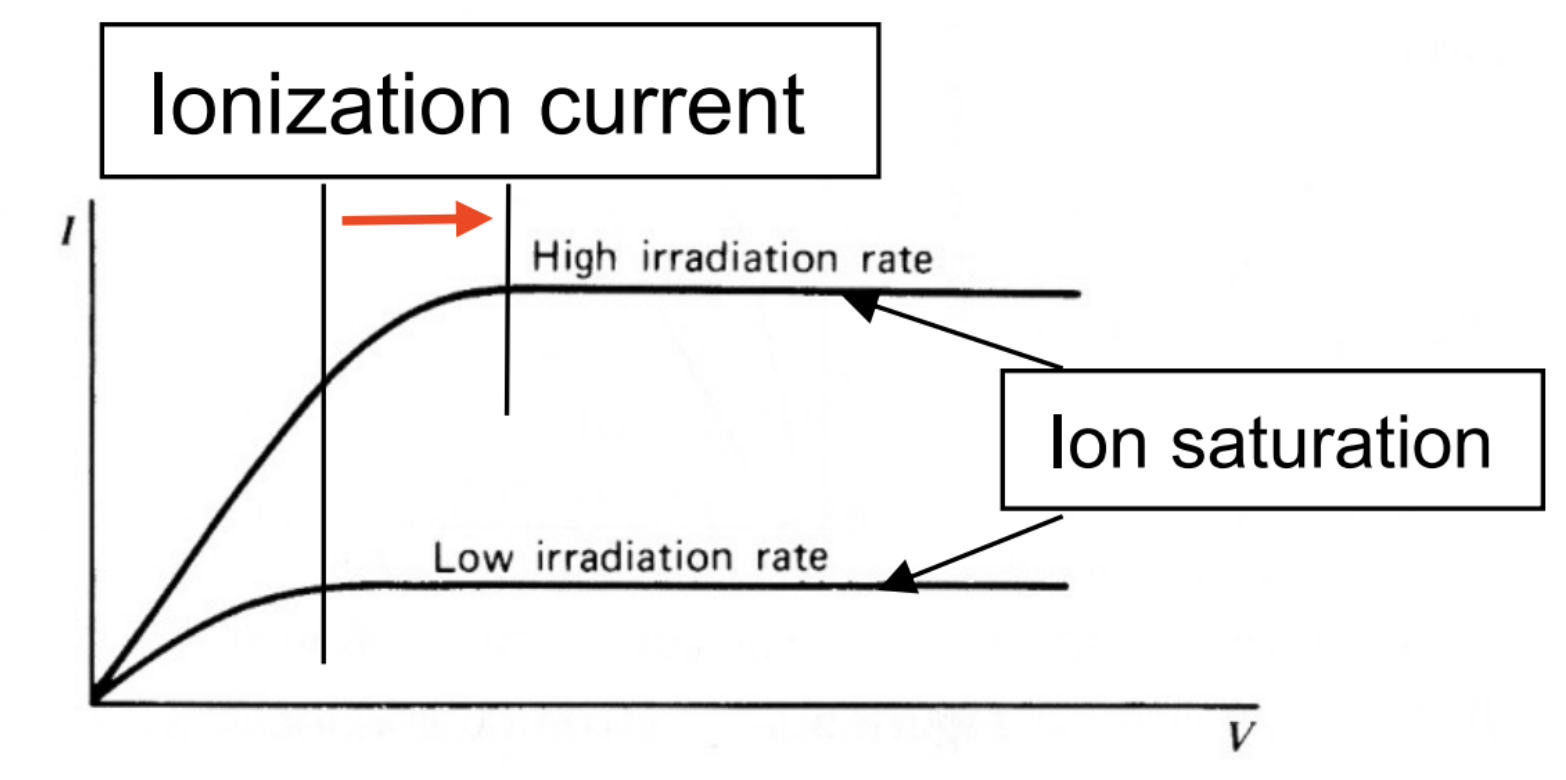
\includegraphics[width=0.5\textwidth]{images/ion_chamber_saturation_current.png}
    \caption{Saturation currents of ion chambers.}
    \label{fig:ion_chamber_saturation_current}
\end{figure}
\subsubsection{Pulse Mode Operation}

\subsubsection{Energy Resolution and the Fano Factor}
Note that the following calculation methods of energy resolution and the usage of the Fano factor are not exclusive to the context of pulse-mode ionization chambers, but will be applied in future chapters, too. 
\subsection{Proportional Counter}
\subsubsection{Operation}

\subsubsection{Fill Gas and Quenching}

\subsubsection{Applications}

\subsection{Geiger-Müller Counter}
\subsubsection{Operation}
\subsubsection{Fill Gas and Quenching}
\subsubsection{Applications}
\subsection{Position-Sensitive Detection}